\section{Identification}
\label{sec:identification}

Let $d_{V_j}$ denote the coordinate dimension of $V_j$. Fix a user-specified output dimension $d_{Z_j}\le d_{V_j}$. Let $\epsilon_j\sim\operatorname{Unif}(0,1)$ be independent of $(U,V_j,W_j,A,Y(0),Y(1))$. For a measurable representation function, define
\begin{align}
\phi_j:\mathcal V_j\times[0,1]\longrightarrow\mathbb R^{d_{Z_j}},
\qquad
Z_j\triangleq\phi_j(V_j,\epsilon_j).
\end{align}
The deterministic case is included when $\phi_j$ ignores its second input. Let $\Phi_j$ denote a prespecified class of such representation functions.

\subsection{Assumptions}
\label{sec:identification-assumptions}

\begin{assumption}[Consistency and integrability]
\label{ass:consistency}
For each $a\in\{0,1\}$,
\begin{align}
Y=Y(A),
\qquad
\mathbb E|Y(a)|<\infty.
\label{eq:consistency}
\end{align}
\end{assumption}

Consistency connects the observed outcome $Y$ to the potential outcome corresponding to the treatment actually received. Integrability ensures that the causal means used below are finite.

\begin{assumption}[Latent exchangeability and a common held-out channel]
\label{ass:joint-latent-exchangeability}
\label{ass:held-out-separation}
For each $a\in\{0,1\}$,
\begin{align}
Y(a)&\perp\!\!\!\perp A\mid(U,V_j),
\label{eq:joint-latent-exchangeability}\\
W_j&\perp\!\!\!\perp A\mid(U,V_j).
\label{eq:held-out-separation}
\end{align}
\end{assumption}

\begin{assumption}[Representation overlap]
\label{ass:representation-overlap}
\begin{align}
0<P(A=1\mid Z_j)<1
\qquad\text{almost surely}.
\label{eq:representation-overlap}
\end{align}
\end{assumption}

We then introduce the latent and proxy objects within each representation stratum.

\begin{definition}[Latent and proxy objects within a representation stratum]
\label{def:latent-proxy-objects}
Let $P_{Z_j}$ denote the distribution of $Z_j$. The conditional laws below refer to fixed versions that exist under the maintained probability model. For $P_{Z_j}$-almost every $z$, define
\begin{align}
Q_{a,j,z}&\triangleq\mathcal L(V_j,U\mid A=a,Z_j=z),
\qquad a\in\{0,1\}.
\end{align}
Define the held-out proxy channel by
\begin{align}
K_j(\cdot\mid v,u)
\triangleq
\mathcal L(W_j\mid V_j=v,U=u).
\end{align}
For any probability law $Q$ on $(V_j,U)$, let $\mathcal K_jQ$ denote the probability law on $(X,W_j)$ generated in three steps. First draw $(V_j,U)=(X,W_{-j},U)\sim Q$. Next draw $W_j\sim K_j(\cdot\mid V_j,U)$. Finally retain $(X,W_j)$ and integrate out $(W_{-j},U)$.

For each $a\in\{0,1\}$, define
\begin{align}
\mu_{a,j,z}(v,u)
\triangleq
\mathbb E\{Y(a)\mid V_j=v,U=u,Z_j=z\}.
\end{align}
The admissible law class is
\begin{align}
\mathcal Q_{j,z}
\triangleq
\biggl\{
Q:\;&Q\text{ is a probability law on }(V_j,U),\
Q\ll\mathcal L(V_j,U\mid Z_j=z), \notag\\
&\mathbb E_Q|\mu_{a,j,z}(V_j,U)|<\infty
\text{ for }a\in\{0,1\}
\biggr\}.
\end{align}
For $Q\in\mathcal Q_{j,z}$, write
\begin{align}
\mathbb E_Q\{\mu_{a,j,z}(V_j,U)\}
\triangleq
\int\mu_{a,j,z}(v,u)Q(dv,du).
\end{align}
\end{definition}

The notation $Q\ll\mathcal L(V_j,U\mid Z_j=z)$ means that every event impossible under the stratum law of $(V_j,U)$ is also impossible under $Q$. This domination makes the conditional-law versions well defined under $Q$. Under representation overlap and integrability, the actual arm laws $Q_{0,j,z}$ and $Q_{1,j,z}$ belong to $\mathcal Q_{j,z}$.

\begin{assumption}[Exact outcome-relevant completeness]
\label{ass:outcome-relevant-completeness}
For $P_{Z_j}$-almost every $z$, every $Q,Q'\in\mathcal Q_{j,z}$, and each $a\in\{0,1\}$,
\begin{align}
\mathcal K_jQ=\mathcal K_jQ'
\quad\Longrightarrow\quad
\mathbb E_Q\{\mu_{a,j,z}(V_j,U)\}
=
\mathbb E_{Q'}\{\mu_{a,j,z}(V_j,U)\}.
\label{eq:outcome-relevant-completeness}
\end{align}
\end{assumption}

This condition is imposed on the entire class $\mathcal Q_{j,z}$. It need not imply $Q=Q'$ and therefore does not imply latent balance. On a common domain it is weaker than full mixture injectivity, but it is not uniformly comparable with standard proximal completeness because the operators differ.

\subsection{Exact Cross-View Identification}
\label{sec:exact-cross-view-identification}

Because $Z_j$ is constructed from $V_j$ and the independent variable $\epsilon_j$, the next lemma shows that the two conditional independences in Assumption~\ref{ass:joint-latent-exchangeability} remain valid after additionally conditioning on $Z_j$.

\begin{lemma}[Conditioning safety]
\label{lem:conditioning-safety}
Under Assumption~\ref{ass:joint-latent-exchangeability}, for each $a\in\{0,1\}$,
\begin{align}
\mathbb E\{Y(a)\mid A,V_j,U,Z_j\}
=
\mathbb E\{Y(a)\mid V_j,U,Z_j\},
\label{eq:conditioning-safe-outcome}
\end{align}
and, for every measurable $C$,
\begin{align}
P(W_j\in C\mid A,V_j,U,Z_j)=K_j(C\mid V_j,U).
\label{eq:common-channel-after-z}
\end{align}
\end{lemma}

The lemma is used both to connect observed treatment-arm outcomes to the latent laws and to factorize the held-out proxy distribution.

\begin{definition}[Adjustment functional]
\label{def:adjustment-functional}
Let
\begin{align}
m_{a,j}(z)\triangleq\mathbb E(Y\mid A=a,Z_j=z)
\end{align}
denote a version of the observed conditional outcome mean. Define
\begin{align}
\mathbb E\{|m_{1,j}(Z_j)|+|m_{0,j}(Z_j)|\}<\infty.
\label{eq:adjustment-integrability}
\end{align}
Under this integrability condition, define
\begin{align}
\tau_{Z_j}
\triangleq
\mathbb E\{m_{1,j}(Z_j)-m_{0,j}(Z_j)\}.
\label{eq:adjustment-functional}
\end{align}
\end{definition}

\begin{lemma}[Cross-view factorization]
\label{lem:cross-view-factorization}
For each treatment arm and $P_{Z_j}$-almost every $z$,
\begin{align}
\mathcal L(X,W_j\mid A=a,Z_j=z)=\mathcal K_jQ_{a,j,z}.
\label{eq:cross-view-factorization}
\end{align}
\end{lemma}

\begin{definition}[Exact PROBE balance]
\label{def:exact-cross-view-balance}
The fixed representation satisfies exact PROBE balance when
\begin{align}
(X,W_j)\perp\!\!\!\perp A\mid Z_j.
\label{eq:exact-cross-view-balance}
\end{align}
\end{definition}

Exact balance and Lemma~\ref{lem:cross-view-factorization} imply, for $P_{Z_j}$-almost every $z$,
\begin{align}
\mathcal K_jQ_{1,j,z}=\mathcal K_jQ_{0,j,z}.
\label{eq:balanced-channel-images}
\end{align}

\begin{theorem}[Exact identification under PROBE balance]
\label{thm:exact-cross-view-identification}
Suppose Assumptions~\ref{ass:consistency}--\ref{ass:outcome-relevant-completeness} and equation~\eqref{eq:adjustment-integrability} hold. If $Z_j$ satisfies exact PROBE balance, then, for each $a\in\{0,1\}$,
\begin{align}
\mathbb E\{Y(a)\mid A=1,Z_j\}
=
\mathbb E\{Y(a)\mid A=0,Z_j\}
\quad\text{almost surely},
\label{eq:conditional-mean-exchangeability}
\end{align}
and
\begin{align}
\boxed{\tau_{Z_j}=\tau.}
\label{eq:exact-identification}
\end{align}
\end{theorem}

\begin{remark}[Why copying the representation input is not automatic]
For the non-compressive benchmark $Z_j=V_j$, balance of $X$ is automatic, but held-out balance still requires $W_j\perp\!\!\!\perp A\mid V_j$. Thus copying does not automatically satisfy the observed endpoint.
\end{remark}

\begin{remark}[What is, and is not, identified]
The theorem establishes conditional mean exchangeability, not full conditional independence or equality of the latent arm laws.
\label{rem:no-full-latent-balance}
\end{remark}

\begin{remark}[Attainability]
The theorem is conditional on exact balance and does not guarantee that a map attaining it exists in $\Phi_j$.
\label{rem:exact-attainability}
\end{remark}

\subsection{Approximate Cross-View Bias Bound}
\label{sec:approximate-cross-view-bound}

Let $\kappa_j$ be a bounded, measurable, characteristic kernel on $(X,W_j)$ whose reproducing kernel Hilbert space $\mathcal H_j$ is separable. For probability laws $P,P'$ on $(X,W_j)$, write
\begin{align}
\operatorname{MMD}_{\kappa_j}(P,P')
\triangleq
\|m_j(P)-m_j(P')\|_{\mathcal H_j},
\end{align}
where $m_j(P)=\int\kappa_j(r,\cdot)P(dr)$.

\begin{definition}[Cross-view discrepancy]
\label{def:cross-view-discrepancy}
For $P_{Z_j}$-almost every $z$, define
\begin{align}
\Delta_j(z;\phi_j)
\triangleq
\operatorname{MMD}_{\kappa_j}
\left\{
\mathcal L(X,W_j\mid A=1,Z_j=z),
\mathcal L(X,W_j\mid A=0,Z_j=z)
\right\},
\label{eq:stratum-cross-view-discrepancy}
\end{align}
and define
\begin{align}
D_j(\phi_j)\triangleq\mathbb E\{\Delta_j(Z_j;\phi_j)\}.
\label{eq:aggregate-cross-view-discrepancy}
\end{align}
\end{definition}

\begin{proposition}[Zero discrepancy and exact balance]
\label{prop:zero-discrepancy}
Under representation overlap,
\begin{align}
\boxed{D_j(\phi_j)=0
\quad\Longleftrightarrow\quad
(X,W_j)\perp\!\!\!\perp A\mid Z_j.}
\label{eq:zero-discrepancy-equivalence}
\end{align}
\end{proposition}

The factorization lemma gives, almost everywhere,
\begin{align}
\Delta_j(z;\phi_j)
=
\operatorname{MMD}_{\kappa_j}(\mathcal K_jQ_{1,j,z},\mathcal K_jQ_{0,j,z}).
\label{eq:observed-latent-discrepancy-link}
\end{align}

\begin{assumption}[Uniform outcome-relevant stability]
\label{ass:uniform-stability}
There is a finite $\Gamma_j$ such that, for $P_{Z_j}$-almost every $z$, every $a\in\{0,1\}$, and all $Q,Q'\in\mathcal Q_{j,z}$,
\begin{align}
\left|\mathbb E_Q\{\mu_{a,j,z}\}-\mathbb E_{Q'}\{\mu_{a,j,z}\}\right|
\le
\Gamma_j\operatorname{MMD}_{\kappa_j}(\mathcal K_jQ,\mathcal K_jQ').
\label{eq:uniform-stability}
\end{align}
\end{assumption}

Uniform stability converts a difference between held-out proxy distributions into a common upper bound on the corresponding difference in potential-outcome means.

\begin{theorem}[Approximate cross-view bias bound]
\label{thm:approximate-cross-view-bound}
Under Assumptions~\ref{ass:consistency}--\ref{ass:representation-overlap}, Assumption~\ref{ass:uniform-stability}, and equation~\eqref{eq:adjustment-integrability},
\begin{align}
\boxed{|\tau_{Z_j}-\tau|\le\Gamma_jD_j(\phi_j).}
\label{eq:approximate-cross-view-bound}
\end{align}
\end{theorem}

\begin{remark}[Exact completeness and quantitative stability]
Stability implies exact outcome-relevant completeness, but the converse need not hold.
\label{rem:exact-vs-stability}
\end{remark}

\begin{remark}[Sensitivity interpretation]
For a scientifically specified $\Gamma_j$,
\begin{align}
\tau\in[\tau_{Z_j}-\Gamma_jD_j(\phi_j),\tau_{Z_j}+\Gamma_jD_j(\phi_j)].
\end{align}
\label{rem:sensitivity-interpretation}
\end{remark}

\begin{remark}[Uniformity across representations]
Learning by discrepancy requires a common budget
\begin{align}
\sup_{\phi\in\Phi_j}\Gamma_j(\phi)\le\overline\Gamma_j<\infty.
\label{eq:uniform-candidate-stability}
\end{align}
\label{rem:uniform-across-representations}
\end{remark}

\subsection{Comparison with Existing Proximal Frameworks}
\label{sec:comparison-proximal-frameworks}

Standard proximal causal inference assigns treatment-inducing and outcome-inducing proxy roles and uses bridge equations and completeness \citep{miao2018proxy,tchetgen2024ProximalCausalInference}. PROBE instead holds out $W_j$, constructs $Z_j$ from $V_j$, and links observed balance to causal conclusions through outcome-relevant completeness or stability.

\begin{figure}[t]
\centering
\subfloat[Standard proximal]{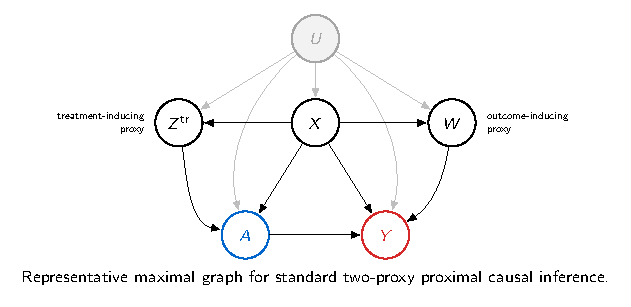
\includegraphics[width=0.46\textwidth]{../figures/2026-08-27-standard-proximal-causal-graph.pdf}}
\hfill
\subfloat[PROBE-compatible]{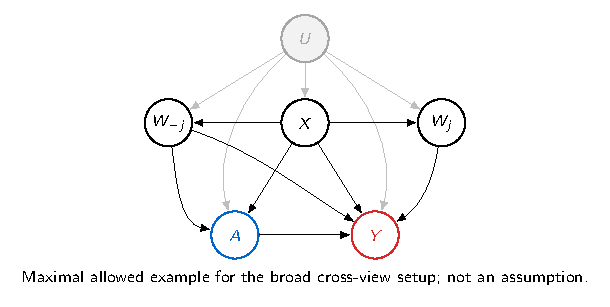
\includegraphics[width=0.46\textwidth]{../figures/2026-08-27-proximal-balancing-maximal-dependence.pdf}}
\caption{Illustrative graphs for standard proximal causal inference and PROBE. The graphs do not by themselves imply the conditional-independence, completeness, or stability assumptions.}
\label{fig:proximal-probe-graphs}
\end{figure}
\FloatBarrier
